\subsection{Unlocking the Magic: The Role of Receiver IF Shift Control!}

\begin{tcolorbox}[colback=gray!10, colframe=black, title=E4C14] What is the purpose of the receiver IF Shift control? 
\begin{enumerate}[label=\Alph*.]
    \item To permit listening on a different frequency from the transmitting frequency
    \item To change frequency rapidly
    \item \textbf{To reduce interference from stations transmitting on adjacent frequencies}
    \item To tune in stations slightly off frequency without changing the transmit frequency
\end{enumerate} \end{tcolorbox}

\subsubsection{Concepts Related to IF Shift Control}

The Intermediate Frequency (IF) shift control is an important feature in radio receivers, particularly in superheterodyne receivers. This concept is fundamental to understanding how radios can demodulate signals and handle various types of interference.

1. \textbf{Superheterodyne Receiver}: This is a type of radio receiver that uses frequency mixing to convert a received signal to a fixed intermediate frequency (IF). This fixed frequency simplifies signal processing and allows for better selectivity and sensitivity.

2. \textbf{Adjacent Frequency Interference}: When multiple stations transmit signals that are close in frequency, they can interfere with one another. This interference leads to degraded audio quality or even complete signal loss for the user. The IF shift control allows the receiver to adjust its operating frequency slightly, mitigating this interference.

3. \textbf{Tuning and Selectivity}: The ability to tune into a desired frequency while keeping interference at bay is crucial. A receiver must be able to differentiate between closely spaced channels. The IF shift achieves this by allowing for small adjustments that can help isolate the desired signal.

\subsubsection{Mathematical Considerations}

While the operation of the IF shift control is based more on electronic principles than pure mathematics, understanding frequency-related calculations can aid in grasping its significance:

- Let \( f_{center} \) be the center frequency of the receiver.
- Let \( \Delta f \) be the necessary shift to effectively eliminate interference from adjacent frequencies.

In practical application, this might involve adjusting the local oscillator frequency:

\[
f_{oscillator} = f_{center} + \Delta f
\]

Where \( \Delta f \) is determined based on the specified adjacent channel separations, ensuring that the receiver can effectively target its desired channel while minimizing unwanted signals.

\subsubsection{Visual Representation}

A simple representation of the concept can be realized with a diagram illustrating frequency ranges around a center frequency:

\begin{center}
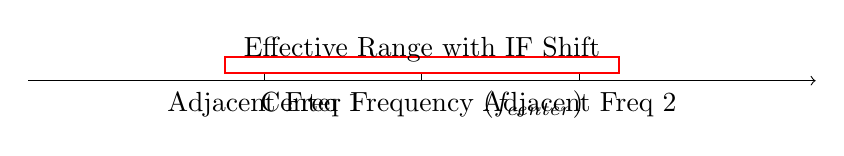
\begin{tikzpicture}
    % Draw the frequency axis
    \draw[->] (0,0) -- (10,0);
    
    % Mark the center frequency
    \draw[dashed] (5,0.1) -- (5,-0.1);
    \node at (5,-0.3) {Center Frequency ($f_{center}$)};
    
    % Indicate adjacent frequencies
    \draw[dashed] (3,0.1) -- (3,-0.1);
    \draw[dashed] (7,0.1) -- (7,-0.1);
    \node at (3,-0.3) {Adjacent Freq 1};
    \node at (7,-0.3) {Adjacent Freq 2};
    
    % Frequency range for IF Shift
    \draw[red, thick] (2.5, 0.3) rectangle (7.5, 0.1);
    \node at (5,0.4) {Effective Range with IF Shift};
\end{tikzpicture}
\end{center}
